%! TEX root = thesis.tex
% vim: ft=tex et sts=2 sw=2

\chapter{Semiclassical physics}
\label{chap04}

In this Chapter we present a quick rundown of the semiclassical approximation as applied to multicomponent waves.
To keep the exposition simple, we will restrict ourselves to wave equations in one variable.
For more detailed descriptions, we refer to the book by \citet{tracy2014}.

% This chapter is a brief discussion of elastic waves.
% In particular, we discuss waves propagating on a filament and shell, both with varying curvatures.
% The equations we derive in this chapter would form the basis of our discussions in the next chapter.

%\section{WKB analysis}

%Consider the differential equation
%%
%\begin{equation}
%  y''(x) + y(x) + \varepsilon \lambda(x) = 0.
%\end{equation}
%%
%Here $\varepsilon$ is a small parameter and suppose we wish to find solutions to this differential equation when $\varepsilon \to 0$.
%This is a \emph{regular perturbation} problem because the general characteristic features of this differential equation, namely the fact that it is second order with two independent solutions remains preserved on setting $\varepsilon = 0$.
%Hence we can attempt to find a solution of the form
%%
%\begin{equation}
%  y(x) = y_0(x) + \varepsilon y_{1}(x) + \varepsilon^{2} y_{2}(x) + \cdots
%\end{equation}
%%
%Putting this in the original differential equation, we can solve it at different orders of $\varepsilon$ to find
%%
%\begin{equation}
%  \begin{aligned}
%    \mathcal{O}(\epsilon^{0}) &: y_{0}''(x) + y_{0}(x) = 0\\
%    \mathcal{O}(\epsilon^{1}) &: y_{1}''(x) + y_{0}(x) = 0
%  \end{aligned}
%\end{equation}
%%

%The WKB method is a method to find solutions to \emph{singularly perturbed} different equations.

%Trouble might occur for instance when

%1) the highest order derivative is multiplied by $\varepsilon$.
%2) the problem totally changes characteristics when the parameter $\varepsilon$ is equal to zero.
%3) the problem is defined on infinite regions.
%4) singular points are present.
%5) the equation models physical processes with several time- or length scales.

%1-5 are called singular perturbation problems.

%In many cases we deal with problem containing boundary layers. We can roughly treat these problems by
%i) letting  we get a good approximation for the outer region.
%ii) rescale the problem to get an inner approximation.
%iii) match inner and outer approximations.

%Singular perturbation is matched asymptotic expansion.

\section{Introduction}

Consider a wave equation of the form
%
\begin{equation}
  \partial_{t}^{2}\Psi(x,t) + \widehat{\mathsf{H}}\Psi(x,t) = 0,
  \label{eq:full_wave_eq}
\end{equation}
%
where $\Psi(x,t)$ is an $N$-component wave field described by a one-dimensional coordinate $x$ and time $t$.
In elastodynamics, $\Psi$ is usually composed of displacements, e.g., for the rod we have $\Psi = (\zeta, u)$, and for the shell we have $\Psi = (\zeta, u, v)$ [see Figs.~\ref{fig:waves}(a) and~\ref{fig:waves}(b)].
Also, $\widehat{\mathsf{H}}$ is taken to be a Hermitian operator in the form of an $N\times N$ matrix, composed solely of spatial derivatives (i.e., powers of $\partial_{x}$) with time-independent coefficients.
Assuming that the waves are time harmonic with frequency $\omega$, i.e., $\Psi(x, t) = \psi(x)e^{\pm i\omega t}$, where $\psi(x)$ is the time-independent part of the wave field, Eq.~\eqref{eq:full_wave_eq} can be recast as
%
\begin{equation}
  \widehat{\mathsf{D}}\psi = 0,\quad \text{with}\enspace \widehat{\mathsf{D}} = \widehat{\mathsf{H}} - \omega^{2}\mathsf{I}_{N},
  \label{eq:ev_problem}
\end{equation}
%
where $\mathsf{I}_{N}$ is the $N\times N$ identity matrix.

If the coefficients of the spatial derivatives that appear in $\widehat{\mathsf{D}}$ are constants, then the eigenmodes $\psi$ are plain waves.
In what follows we assume that these coefficients are slowly varying, with the variation controlled by a single positive parameter $\epsilon \ll 1$, called the \emph{eikonal parameter}.
It is useful to treat $\epsilon$ as an ordering parameter so that we can look for solutions at various orders of $\epsilon$.
To this end, we rescale $x \to \epsilon^{-1}x$ so that a derivative $\partial_{x}$ becomes $\epsilon \partial x$.
With analogy to quantum mechanics, this allows us to recast the derivatives in $\widehat{\mathsf{D}}$ in terms of the wave number/momentum operator $\hat{k} = -i\epsilon \partial_{x}$, with $\epsilon$ playing the role of Planck's constant.
Since we shall be considering $\widehat{\mathsf{D}}$ in the coordinate representation, the position operator $\hat{x} = x$.

\subsection{Wave action}

An equation like Eq.~\eqref{eq:ev_problem} can be derived from a wave action of the form
%
\begin{equation}
  \begin{aligned}
    \mathscr{U}\left[\psi^{*}, \psi\right] &= \frac{1}{2}\bra{\psi}\widehat{\mathsf{D}}\ket{\psi}
  = \frac{1}{2}\int \dd{x}\,\dd{x'}\, \braket{\psi|x}\bra{x}\widehat{\mathsf{D}}\ket{x'}\braket{x'|\psi}\\
                                           &= \frac{1}{2}\int \dd{x}\dd{x'}\, \psi^{*}_{j}(x)\,\widehat{\mathsf{D}}_{jk}(x, x')\,\psi_{k}(x').
  \label{eq:wave_action}
  \end{aligned}
\end{equation}
%
Above we have inserted the resolution of identity $\int \dd{x}\,\ket{x}\bra{x} = 1$ in appropriate places to express $\mathscr{U}$ in terms of $\psi$ and its conjugate $\psi^{*}$.
Also, we have made the product between the matrix operator $\widehat{\mathsf{D}}$ and the wave vector $\psi$ explicit, with $\braket{x|\widehat{\mathsf{D}}_{jk}|x'} = \widehat{\mathsf{D}}_{jk}(x, x')$ being the matrix element of $\widehat{\mathsf{D}}_{jk}$ in the position basis.
Varying $\mathscr{U}[\psi^{*}, \psi]$ with respect to $\psi^{*}$ gives the eigenvalue problem, Eq.~\eqref{eq:ev_problem}.

For later use, we also note that $\mathscr{U}$ can also be written as
%
\begin{equation}
  \begin{aligned}
    \mathscr{U}\left[\psi^{*}, \psi\right] &= \tfrac{1}{2}\int \dd{x}' \braket{\psi_{\mu}|x'}\bra{x'}\widehat{\mathsf{D}}_{\mu\nu}\ket{\psi_{\nu}}
= \tfrac{1}{2}\int \dd{x}' \bra{x'}\widehat{\mathsf{D}}_{\mu\nu}\ket{\psi_{\nu}} \braket{\psi_{\mu}|x'}\\
&= \tfrac{1}{2}\int \dd{x}' \bra{x'}\widehat{\mathsf{D}}_{\mu\nu}\widehat{\mathsf{W}}_{\nu\mu}\ket{x'} = \tr\left(\widehat{\mathsf{D}}_{\mu\nu}\widehat{\mathsf{W}}_{\nu\mu}\right).
  \label{eq:wave_action_trace_form}
  \end{aligned}
\end{equation}
%

In order to solve Eq.~\eqref{eq:ev_problem} at various orders of $\epsilon$, it is convenient to make use of Weyl calculus, which allows one to map differential operators that are functions of $\hat{x}$ and $\hat{k}$ to ordinary functions, called Weyl symbols, defined on an $x$-$k$ phase space, and vice versa~\cite{chaichian2001,cohen2012}.
For the purposes of this chapter, the following simple rules suffice to convert operators to symbols:
%
\begin{equation}
  f(x) \to f(x),\enspace
  g(\hat{k}) \to g(k),\enspace\text{and}\enspace
  f(x)g(\hat{k}) \to f(x)g(k) + \frac{i\epsilon}{2}f'(x)g'(k) + \mathcal{O}(\epsilon^{2}).
  \label{eq:weylrules}
\end{equation}
%
Above, $f$ and $g$ are functions of $x$ and $\hat{k}$, with the primes denoting derivatives.
Converting each entry of the matrix operator $\widehat{\mathsf{D}}$ into a Weyl symbol, we get the $N\times N$ dispersion matrix $\mathsf{D}$, which we express in various orders of $\epsilon$ as $\mathsf{D} = \mathsf{D}^{(0)} + \epsilon\mathsf{D}^{(1)} + \mathcal{O}(\epsilon^{2})$.

The Wigner tensor $\mathsf{W}_{kj}$ is defined as the symbol of the density operator $\widehat{\mathsf{W}} = \ket{\psi}\bra{\psi}$ with kernel $\widehat{\mathsf{W}}_{kj}(x',x) = \psi_{k}(x')\psi_{j}^{*}(x)$.
%
\begin{equation}
  \mathsf{W}_{kj}(x, k) = \int \dd{s}\, e^{-iks/\epsilon}\, \psi_{k}\left(x + \tfrac{1}{2}s\right)\psi^{*}_{j}\left(x - \tfrac{1}{2}s\right).
\end{equation}
%
By inverting the above expression, and setting $x + \frac{1}{2}s \to x'$ and $x- \frac{1}{2}s \to x$, we can write the kernel of the density operator in terms of its Weyl symbol as
%
%\begin{equation}
%  \psi_{k}\left(x + \tfrac{1}{2}s\right) \psi^{*}_{j}\left(x - \tfrac{1}{2}s\right) = \frac{1}{2\pi \epsilon} \int \dd{k}\, e^{iks/\epsilon}\,\mathsf{W}_{kj}(x, k).
%\end{equation}
%%
%so that
%
\begin{equation}
  \psi_{k}(x') \psi^{*}_{j}(x) = \frac{1}{2\pi \epsilon} \int \dd{k}\, e^{ik(x' -x)/\epsilon}\,\mathsf{W}_{kj}\left[\tfrac{1}{2}(x' + x), k\right].
  \label{eq:density_operator}
\end{equation}
%
In a similar fashion, we find
%
\begin{equation}
  \widehat{\mathsf{D}}_{jk}(x, x') = \frac{1}{2\pi\epsilon} \int \dd{l}\, e^{il(x -x')/\epsilon}\,\mathsf{D}_{jk}\left[\tfrac{1}{2}(x + x'), l\right].
  \label{eq:Dhat_integral}
\end{equation}
%
Putting Eq.~\eqref{eq:Dhat_integral} and \eqref{eq:density_operator} in Eq.~\eqref{eq:wave_action}, we arrive at
%
\begin{equation}
  \mathscr{U} = \frac{1}{(2\pi\epsilon)^{2}}\int \dd{x}\,\dd{x'}\,\dd{k}\,\dd{l}\, e^{i(l-k)(x -x')/\epsilon}\,\mathsf{W}_{kj}\left[\tfrac{1}{2}(x' + x), k\right]\, \mathsf{D}_{jk}\left[\tfrac{1}{2}(x + x'), l\right].
\end{equation}
%
Performing the change of variables $x \to \frac{1}{2}(x + x')$ and $x' \to x - x'$, which carries a Jacobian factor of unity, we arrive at
%
\begin{equation}
  \begin{aligned}
    \mathscr{U} &= \frac{1}{(2\pi\epsilon)^{2}}\int \dd{x}\,\dd{x'}\,\dd{k}\,\dd{l}\, e^{i(l-k)x'/\epsilon}\,\mathsf{W}_{kj}(x, k)\, \mathsf{D}_{jk}(x, l)\\
                &= \frac{1}{2\pi\epsilon}\int \dd{x}\,\dd{k}\,\mathsf{W}_{kj}(x,k)\,\mathsf{D}_{jk}(x, k).
  \end{aligned}
  \label{eq:wave_action_symbol_form}
\end{equation}
%

The curious reader may wonder if the above equation is incorrect, in light of Eq.~\eqref{eq:wave_action_trace_form}, where we have expressed $\mathscr{U}$ as the trace of the operator $\widehat{O} = \widehat{\mathsf{D}}_{\mu\nu}\widehat{\mathsf{W}}_{\nu\mu}$.
In terms of its symbol, the trace of an operator $\widehat{O}$ is
%
\begin{equation}
  \tr\widehat{O} = \frac{1}{2\pi\epsilon} \int \dd{x}\,\dd{k}\, O(x, k),
\end{equation}
%
so that $\mathscr{U}$ must be
%
\begin{equation}
  \mathscr{U} = \frac{1}{4\pi\epsilon}\int \dd{x}\,\dd{k}\, D_{\mu\nu}(x,k)e^{i\mathcal{L}}W_{\nu\mu}(x, k),
\end{equation}
%
where we have used the Moyal formula to write the symbol $O$ in terms of the symbols of $\mathsf{D}_{\mu\nu}$ and $\mathsf{W}_{\nu\mu}$.
The problem here is a bit subtle---the resolution being that each correction term in the Moyal series can be expressed as divergence of a vector field in the $(x, k)$ phase space~\cite[Problem 3.16]{tracy2014}.
Hence, using the divergence theorem, integral over the correction terms vanish for well behaved wave fields.
Thus, only the first term in the Moyal series remain, and we get Eq.~\eqref{eq:wave_action_symbol_form} again.
So far there has been no approximations involved and Eq.~\eqref{eq:wave_action_symbol_form} is exact to all orders of the eikonal parameter.

Returning to our main problem, i.e., to employ the semiclassical approximation to solve Eq.~\eqref{eq:ev_problem}, we will proceed as follows: (i) insert the eikonal ansatz; (ii) expand the action to the lowest order in the eikonal parameter and form the \emph{reduced action} $\mathscr{U}_{\text{R}}$; (iii) extract the semiclassical equations of motions by varying the reduced action.

\subsubsection*{Reduced wave action}

We look for \emph{eikonal} solutions to Eq.~\eqref{eq:ev_problem} of the form $\psi(x) = A(x)e^{iS(x)/\epsilon}$, where the amplitude $A(x)$ is an $N$-component spinor with complex components, and $S(x)$ is a rapidly varying phase, playing the role of an action.
To this end we set $\psi_{\mu} = A_{\mu}e^{iS(x)/\epsilon}$ in Eq.~\eqref{eq:wave_action_symbol_form} to obtain%
%
\begin{equation}
    \mathsf{W}_{\nu\mu}(x, k) = \int \dd{r}\,e^{ikr/\epsilon} A_{\nu}\left(x + \tfrac{1}{2} r\right)A_{\mu}^{*}\left(x - \tfrac{1}{2} r\right)\exp\left\{\frac{i}{\epsilon}\left[S\left(x + \tfrac{1}{2} r\right) - S\left(x - \tfrac{1}{2} r\right)\right]\right\}.
\end{equation}
%
Next, we set $r \to \epsilon r$ and expand the amplitude $A_{\nu}(x + \frac{1}{2}\epsilon r) = A_{\nu}(x) + \frac{1}{2}(\partial_{x}A_{\nu})\epsilon r + \mathcal{O}(\epsilon^{2})$ and the phase $S(x + \frac{1}{2}\epsilon r) = S(x) + \frac{1}{2}[\partial_{x}S(x)]\epsilon r + \mathcal{O}(\epsilon^{2})$ to obtain
%
\begin{equation}
  \begin{aligned}
    \mathsf{W}_{\nu\mu}(x, k) &= \epsilon\int \dd{r}\,e^{ikr} A_{\nu}(x)A_{\mu}^{*}(x)\exp\left\{ir\left[\partial_{x}S(x) - k\right]\right\} + \mathcal{O}(\epsilon^{2}) \\
                        &= 2\pi\epsilon A_{\nu}(x)A^{*}_{\mu}(x)\delta\left[k - \partial_{x}S(x)\right] + \mathcal{O}(\epsilon^{2}).
  \end{aligned}
\end{equation}
%
Putting the ``reduced'' Wigner tensor in Eq.~\eqref{eq:wave_action_symbol_form}, we find
%
\begin{equation}
  \mathscr{U} = \tfrac{1}{2}\int \dd{x}\, \mathsf{D}_{\mu\nu}\left[x, k=\partial_{x}S(x)\right]A_{\nu}(x)A^{*}_{\mu}(x) + \mathcal{O}(\epsilon^{2}).
  \label{eq:wave_action_reduced_1}
\end{equation}
%
Next, we perform a spectral decomposition of the symbol matrix $\mathsf{D}_{\mu\nu}(x, k)$ and write it in terms of its eigenvectors $\tau_{a}$ and eigenvalues $\lambda_{a}$ as
%
\begin{equation}
  \mathsf{D}_{\mu\nu}(x, k) = \sum_{a} \lambda_{a}(x, k) \tau_{\mu, a}(x, k) \tau_{\nu, a}^{*}(x, k).
\end{equation}
%
Using this in Eq.~\eqref{eq:wave_action_reduced_1}, and defining $B_{a} = \tau_{\nu, a}^{*}A_{\nu} = \braket{\tau_{a}|A}$, which is the projection of the amplitude $A_{\nu}$ along the direction of the polarization vector $\tau_{a}$, we finally arrive at the reduced action
%
\begin{equation}
  \mathscr{U}_{\text{R}}\left[B_{a}, S\right] = \tfrac{1}{2} \sum_{a} \int \dd{x}\, \lambda_{a}(x,k) \abs{B_{a}(x, k)}^{2},
  \quad\text{with}\quad
  k = \partial_{x}S(x).
\end{equation}
%

Variation with respect to the amplitude $B_{a}$ yields
%
\begin{equation}
  \lambda_{a}(x, k) B_{a}(x, k) = 0.
\end{equation}
%
For nontrivial solutions with $B_{a}(x, k) \neq 0$, we must then have
%
\begin{equation}
  \lambda_{a}\left[x, \partial_{x}S(x)\right] = 0,
\end{equation}
%
which is the eikonal equation.
This equation is nothing but the Hamilton--Jacobi equation with $S(x)$ playing the role of the classical action.
The corresponding Hamilton's equations read
%
\begin{equation}
  \frac{\dd{x}}{\dd{\sigma}} = \partial_{k}\lambda_{a}(x, k)
  \quad\text{and}\quad
  \frac{\dd{k}}{\dd{\sigma}} = -\partial_{x}\lambda_{a}(x, k),
\end{equation}
%
where $\sigma$ is some parameter that parameterizes the rays $[x(\sigma), k(\sigma)]$ in the phase space.

A vanishing eigenvalue $\lambda$ and the associated normalized eigenvector $\tau$ describes different wave types or ``polarizations'' represented by Eq.~\eqref{eq:ev_problem}.
By a polarization we mean a linear subspace of the total wave field that is usually of a distinct physical nature, e.g., flexural waves on a curved rod.
Semiclassical approximation breaks down near points where more than one eigenvalues of $\mathsf{D}^{(0)}$ simultaneously vanish, precipitating an exchange of energy and mode conversion between waves of different polarizations~\cite{tracy2014}.

In the absence of mode conversion, the vanishing eigenvalues of $\mathsf{D}^{(0)}$ also serve as the \emph{ray Hamiltonian} of waves of a specific polarization.
 This leads us to the phase-space representation of waves as rays that satisfy the Hamilton's equations
%
\begin{equation}
  \dot{x} = \partial_{k} \lambda(x, k;\, \omega) = \left\{x, \lambda\right\}
  \quad\text{and}\quad
  \dot{k} = -\partial_{x} \lambda(x, k;\, \omega) = \left\{k, \lambda\right\},
\end{equation}
%
where the overdot denotes derivatives with respect to a parameter that parameterizes the rays and $\left\{\cdot, \cdot\right\}$ is the $x$-$k$ Poisson bracket.
Since the waves we consider propagate in a one-dimensional space, these rays are identical to the level curve defined by $\lambda(x, k; \omega) = 0$.

In higher dimensions, solving the Hamilton-Jacobi equations can be nontrivial.
However, in one-dimensions, it is always theoretically possible to solve for $k(x)$ from $\lambda_{a}(x, k) = 0$.
% TODO: Tori... quantization, more stuff about Hamilton-Jacobi equations.
Variation with respect to the phase $S(x)$ yields the amplitude transport equation
%
\begin{equation}
  \frac{\dd}{\dd{x}}\left\{\partial_{k}\left[\lambda_{a}(x, k)\abs{B_{a}(x, k)}^{2}\right]\right\} = 0
\end{equation}
%
so that%
\footnote{Here we have ignored the term $\lambda_{a}(x, k)\partial_{k}\abs{B_{a}(x,k)}^{2}$, which trivially vanishes as $\lambda_{a}(x, k) = 0$ on an orbit.}
$\partial_{k}\lambda_{a}(x, k)\abs{B_{a}(x, k)}^{2} = C$ (constant) and
%
\begin{equation}
  B_{a}(x) = \frac{C}{\sqrt{\partial_{k}\lambda_{a}(x, k)}}.
\end{equation}
%
Clearly, $B_{a}$ becomes ill defined at caustics where $\dot{x} = \partial_{k}\lambda_{a}(x, k) = 0$ and the eikonal form of the solutions breaks down.

%Employing the eikonal ansatz, at $\mathcal{O}(\epsilon^{0})$, we find the matrix equation $\mathsf{D}^{(0)}A = 0$.
%To satisfy this equation, at least one of the $N$ eigenvalues of $\mathsf{D}^{(0)}$, say $\lambda(x, k;\, \omega)$, must vanish so that $\det \mathsf{D}^{(0)}(x, k; \omega) = 0$.
%A vanishing eigenvalue $\lambda$ and the associated normalized eigenvector $\tau$ describes different wave types or ``polarizations'' represented by Eq.~\eqref{eq:ev_problem}.
%By a polarization we mean a linear subspace of the total wave field that is usually of a distinct physical nature, e.g., flexural waves on a curved rod.
%Semiclassical approximation breaks down near points where more than one eigenvalues of $\mathsf{D}^{(0)}$ simultaneously vanish, precipitating an exchange of energy and mode conversion between waves of different polarizations~\cite{tracy2014}.

%In the absence of mode conversion, the vanishing eigenvalues of $\mathsf{D}^{(0)}$ also serve as the \emph{ray Hamiltonian} of waves of a specific polarization.
% This leads us to the phase-space representation of waves as rays that satisfy the Hamilton's equations
%%
%\begin{equation}
%  \dot{x} = \partial_{k} \lambda(x, k;\, \omega) = \left\{x, \lambda\right\}
%  \quad\text{and}\quad
%  \dot{k} = -\partial_{x} \lambda(x, k;\, \omega) = \left\{k, \lambda\right\},
%\end{equation}
%%
%where the overdot denotes derivatives with respect to a parameter that parameterizes the rays and $\left\{\cdot, \cdot\right\}$ is the $x$-$k$ Poisson bracket.
%Since the waves we consider propagate in a one-dimensional space, these rays are identical to the level curve defined by $\lambda(x, k; \omega) = 0$.
%%
% \begin{figure}
%   \begin{center}
%     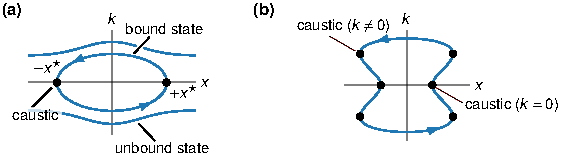
\includegraphics{localization/caustic.pdf}
%   \end{center}
%   \caption{%
%     (a) In phase space, bound states are represented by rays in the form of closed orbits, which is analogous to that of a bound particle oscillating between two classical turning points ($\pm x^{\star}$ in the cartoon).
%     Other trajectories represent unbound states.
%     (b) A bound state represented by a ``peanut''-shaped orbit has six caustics.%
%   }
%   \label{fig:caustic}
% \end{figure}

%%
%\begin{equation}
%\gamma_{\text{G}} = \oint \dd{\sigma}\, \dot{\gamma}_{\text{G}} = i\oint \dd{\sigma}\,\left\langle{\tau_{\alpha}}\middle|\dot{\tau}_{\alpha}\right\rangle =
%  i\oint \dd\xi\cdot\left\langle{\tau_{\alpha}}\middle|\nabla_{\xi}\tau_{\alpha}\right\rangle,
%\end{equation}
%%
%where $\xi = (x, k)$ denotes the ``parameters'' that are being varied.

%%In Appendix~\ref{app:additional_phase} we prove that $\gamma_{\text{G}}$ vanishes if the relative phases between the components of the eigenvector $\tau_{\alpha}$ are constants.
%%The second (non-geometric) phase $\gamma_{\text{NG}}$ need not vanish in such a situation, however.
%Instead of explicitly accounting for the extra phase $\gamma$ in the quantization rule, we could have diagonalized the wave equation at various orders of $\epsilon$~\cite{littlejohn1991,littlejohn1991a,weigert1993,venaille2023}.
%During such a procedure, terms proportional to $\dot{\gamma}_{\text{G}}$ and $\dot{\gamma}_{\text{NG}}$ naturally appear in the ray Hamiltonian $\lambda$ as a first-order correction.
%Despite the elegance of the method, we do not use it in our analysis.
%This is because, as we discuss in Appendix~\ref{app:additional_phase}, for both the problems we consider, the extra phases vanish.


\section{Intermission: diagonalizing multicomponent operators}

Consider a Hermitian linear differential operator $\widehat{\mathsf{D}}$ satisfying the wave equation
%
\begin{equation}
  \widehat{\mathsf{D}}\Psi = 0,
\end{equation}
%
where $\Psi$ is a multicomponent wave field.
%
We want to find a unitary operator ${\mathsf{U}}$ such that%
\footnote{It should be emphasized that diagonalizability and unitarity are independent. For instance, let $\mathsf{U}$ be the usual unitary matrix that diagonalizes a matrix $\mathsf{D}$.
  If $\Sigma$ is some nonzero diagonal matrix, not necessarily unitary, then $(\Sigma^{\dagger}\mathsf{U}^{\dagger})\mathsf{D}(\mathsf{U}\Sigma)$ is a diagonal matrix, which follows from the fact that the product of diagonal matrices is diagonal.
  In this sense $\mathsf{U}\Sigma$ can diagonalize $\mathsf{D}$ without being unitary.}
%
\begin{equation}
  \widehat{\mathsf{U}}^{\dagger}\widehat{\mathsf{D}}\widehat{\mathsf{U}} = \hat{\Lambda}\label{eq:diagonalization}
\end{equation}
%
is a diagonal operator.
Clearly, this equivalent to demanding that $\widehat{\mathsf{D}}\widehat{\mathsf{U}} = \widehat{\mathsf{U}}\hat{\Lambda}$.
If we can find such an operator and solve the decoupled set of equations given by $\hat{\Lambda}\Phi = 0$ somehow,
the solutions to the original equation can then be recovered from $\Phi$ using $\Psi = \widehat{\mathsf{U}}\Phi$.
However, Eq.~\eqref{eq:diagonalization} is an equation involving operators and standard linear algebra methods do not (directly) help in finding the unitary operator $\widehat{\mathsf{U}}$.

We start by finding the symbol form of the following two equations.
%
\begin{equation}
  \begin{aligned}
    \widehat{\mathsf{D}}\widehat{\mathsf{U}} &= \widehat{\mathsf{U}}\hat{\Lambda}\\
    \widehat{\mathsf{U}}^{\dagger}\widehat{\mathsf{U}} &= \mathsf{I}_{n}.
  \end{aligned}
\end{equation}
%
Here we assume that the operators $\widehat{\mathsf{D}}$, $\widehat{\mathsf{U}}$, and $\hat{\Lambda}$ have some problem-relevant ordering parameter $\epsilon$ so that we can expanded the operators (and their symbols) in terms of $\epsilon$.%
\footnote{In their papers, Littlejohn and coworkers~\cite{littlejohn1991,weigert1993} assume that $\widehat{\mathsf{D}}$ is \emph{not} ordered in $\epsilon$, i.e., $\widehat{\mathsf{D}} = \widehat{\mathsf{D}}_{0}$.
  This might seem confusing at first since the parameter $\epsilon$ must appear somewhere in the problem.
  The thing is that very often, $\epsilon$ appears as a factor to a spatial derivative operator, e.g., $-i\epsilon\partial_{x}$, which put together becomes a momentum operator that doesn't have further $\epsilon$ dependence.
  Of course, $\widehat{\mathsf{D}}$ could have further nontrivial dependence on $\epsilon$, which is a more general situation, and the one we want to consider here.
}
%
\begin{equation}
  \begin{aligned}
    \widehat{\mathsf{D}} &= \widehat{\mathsf{D}}_{0} + \epsilon\widehat{\mathsf{D}}_{1} + \epsilon^{2}\widehat{\mathsf{D}}_{2} + \cdots\\
    \widehat{\mathsf{U}} &= \widehat{\mathsf{U}}_{0} + \epsilon\widehat{\mathsf{U}}_{1} + \epsilon^{2}\widehat{\mathsf{U}}_{2} + \cdots\\
    \hat{\Lambda} &= \hat{\mathsf\Lambda}_{0} + \epsilon\hat{\mathsf\Lambda}_{1} + \epsilon^{2}\hat{\mathsf\Lambda}_{2} + \cdots
  \end{aligned}
  \qquad\text{and}\qquad
  \begin{aligned}
    {\mathsf{D}} &= {\mathsf{D}}_{0} + \epsilon{\mathsf{D}}_{1} + \epsilon^{2}{\mathsf{D}}_{2} + \cdots\\
    {\mathsf{U}} &= {\mathsf{U}}_{0} + \epsilon{\mathsf{U}}_{1} + \epsilon^{2}{\mathsf{U}}_{2} + \cdots\\
    {\Lambda} &= {\mathsf\Lambda}_{0} + \epsilon{\mathsf\Lambda}_{1} + \epsilon^{2}{\mathsf\Lambda}_{2} + \cdots
  \end{aligned}
\end{equation}
%
Because the Weyl correspondence preserves Hermiticity, $\mathsf{D}$ is a Hermitian matrix.
We demand that $\Lambda$ remains diagonal at all orders of $\epsilon$.
We then use the Moyal star product to find the symbol form at different orders of $\epsilon$.
At $\mathcal{O}(\epsilon^0)$ we find $\mathsf{D}_{0}\mathsf{U}_{0} = \mathsf{U}_{0}\Lambda_{0}$ and $\mathsf{U}_{0}^{\dagger}\mathsf{U}_{0} = \mathsf{I}_{n}$, which is equivalent to
%
\begin{equation}
  \mathsf{U}_{0}^{\dagger}\mathsf{D}_{0}\mathsf{U}_{0} = \Lambda_{0}.\label{eq:omega0}
\end{equation}
%
Since we demand $\Lambda_{0}$ to be diagonal, this is the usual linear-algebra problem of diagonalizing the matrix $\mathsf{D}_{0}$.
We thus deduce that columns of the lowest order symbol $\mathsf{U}_{0}$ is composed of eigenvectors $\bm{\tau}^{(i)}$ with eigenvalues $\lambda_{0}^{(i)}$ satisfying $\mathsf{D}_{0}\bm{\tau}^{(i)} = \lambda_{0}^{(i)}\bm{\tau}^{(i)}$:
%
\begin{equation}
  \mathsf{U}_{0} =
  \begin{pmatrix}
    \bm{\tau}^{(1)} & \bm{\tau}^{(2)} & \cdots & \bm{\tau}^{(n)}
  \end{pmatrix},
\end{equation}
%
and $\Lambda_{0}$ is the diagonal matrix composed of the eigenvalues $\lambda^{(i)}$.

At $\mathcal{O}(\epsilon^{1})$, demanding $\mathsf{D}\mathsf{U} = \mathsf{U}\Lambda$ gives us
%
\begin{equation}
\mathsf{D}_{1}\mathsf{U}_{0} + \mathsf{D}_{0}\mathsf{U}_{1} + \frac{i}{2}\left\{\mathsf{D}_{0}, \mathsf{U}_{0}\right\} =
  \mathsf{U}_{1}\Lambda_{0} + \mathsf{U}_{0}\Lambda_{1} + \frac{i}{2}\left\{\mathsf{U}_{0}, \Lambda_{0}\right\}.
\end{equation}
%
Multiplying from the left by $\mathsf{U}_{0}^{\dagger}$ and making use of $\mathsf{U}_{0}^{\dagger}\mathsf{D} = \Lambda_{0}\mathsf{U}_{0}^{\dagger}$, we get the $\mathcal{O}(\epsilon)$ correction%
\footnote{For further higher-order corrections to $\Lambda$, see Eq.~(19) of Ref.~\cite{weigert1993}.
Equation~\eqref{eq:omega1} is almost identical to Eqs.~(22)--(24) of Ref.~\cite{venaille2023}, except for the commutator term.
In Ref.~\cite{venaille2023} the commutator term vanishes trivially since $\Lambda_{0}$ is considered to be a scalar.}
%
\begin{equation}
  \Lambda_{1} = \left(\mathsf{U}_{0}^{\dagger}\mathsf{D}_{1}\mathsf{U}_{0} +
  \frac{i}{2}\mathsf{U}_{0}^{\dagger}\left\{\mathsf{D}_{0},\Lambda_{0}\right\} - \frac{i}{2}\mathsf{U}_{0}^{\dagger}\left\{\mathsf{U}_{0},\Lambda_{0}\right\}\right) + \left[\Lambda_{0},\mathsf{U}_{0}^{\dagger}\mathsf{U}_{1}\right].
  \label{eq:omega1}
\end{equation}
%
Above $[~,~]$ denotes the matrix commutator.
We can find $\mathsf{U}_{0}$ and $\Lambda_{0}$ by diagonalizing $\mathsf{D}_{0}$.
The matrix $\mathsf{D}_{1}$ (if it is nonzero) can be found by expanding the symbol matrix $\mathsf{D}$.
But that will not let us find $\Lambda_{1}$ since we still need $\mathsf{U}_{1}$ to evaluate the commutator term $[\Lambda_{0},\mathsf{U}_{0}^{\dagger}\mathsf{U}_{1}]$.
To proceed, we recall that we want $\Lambda$ to be diagonal at all order, which means that $\Lambda_{1}$ must be a diagonal matrix as well.
The $\alpha\beta$th entry of the commutator term evalutes to
%
\begin{equation}
%  \begin{aligned}
    \left[\Lambda_{0},\mathsf{U}_{0}^{\dagger}\mathsf{U}_{1}\right]_{\alpha\beta} = %\Lambda_{0,\alpha\gamma}\left(\mathsf{U}_{0}^{\dagger}\mathsf{U}_{1}\right)_{\gamma\beta} -
  %\left(\mathsf{U}_{0}^{\dagger}\mathsf{U}_{1}\right)_{\alpha\gamma}\Lambda_{0,\gamma\beta}\\
    %&= \lambda_{0}^{(i)}\delta_{\alpha\gamma}\left(\mathsf{U}_{0}^{\dagger}\mathsf{U}_{1}\right)_{\gamma\beta}
  %-\left(\mathsf{U}_{0}^{\dagger}\mathsf{U}_{1}\right)_{\alpha\gamma} \lambda_{0}^{(k)}\delta_{\gamma\beta}\\
    \left[\lambda_{0}^{(i)} - \lambda_{0}^{(j)}\right]\left(\mathsf{U}_{0}^{\dagger}\mathsf{U}_{1}\right)_{\alpha\beta},
%  \end{aligned}
    \label{eq:diagonal}
\end{equation}
%
where we have made use of the fact that $\Lambda_{0}$ is diagonal with $\alpha\beta$th entry $\Lambda_{0,\alpha\beta} = \lambda_{0}^{(i)}\delta_{\alpha\beta}$.
And we see that the diagonal entries (with $\alpha=\beta$) of the commutator vanish.
So the commutator term does not contribute towards the diagonal entries of $\Lambda_{1}$ and we can find the $\mathcal{O}(\epsilon^{1})$ correction $\lambda_{1}$ by carefully evaluating diagonal entries of the remaining terms in the RHS of Eq.~\fixme.
Before we do that, we need to discuss the role of the commutator term further.
In fact, without this crucial term, the expansion will break down.

\subsection{Role of the commutator term}

None of our arguments so far guarantees that $\Lambda_{1}$ is diagonal.
In fact, the off-diagonal entries of four matrices in the RHS of Eq.~\eqref{eq:omega1} is generally not equal to zero.
The only way for $\Lambda_{1}$ to be diagonal then is if these off-diagonal entries somehow cancel each other.
We don't have the freedom to choose the off-diagonal entries in the first three terms since they only involve the matrices $\mathsf{U}_{0}$ and $\Lambda_{0}$, both of which are constrained by Eq.~\eqref{eq:omega0}.
However, the commutator term involves the matrix $\mathsf{U}_{1}$, which is something we haven't found yet.
At the same time, $\mathsf{U}_{1}$ isn't a completely arbitrary matrix because on demanding unitarity of $\mathsf{U}$ at $\mathcal{O}(\epsilon)$ we get an additional equation that puts constraints on $\mathsf{U}_{1}$:
%
\begin{equation}
  \mathsf{U}_{0}^{\dagger}\mathsf{U}_{1} + \mathsf{U}_{1}^{\dagger}\mathsf{U}_{0} + \frac{i}{2}\left\{\mathsf{U}_{0}^{\dagger}, \mathsf{U}_{0}\right\}= 0.
  \label{eq:unitarity}
\end{equation}
%
This equation isn't good enough to determine $\mathsf{U}_{1}$ completely, which is good for us since that gives us some freedom in choosing the off-diagonal elements of the commutator term in the way we want.
To simplify the commutator term we first define $\mathsf{X} = \mathsf{U}_{0}^{\dagger}\mathsf{U}_{1}$, and from the previous equation we have
%
\begin{equation}
  \mathsf{X} + \mathsf{X}^{\dagger} = -\frac{i}{2}\left\{\mathsf{U}_{0}^{\dagger}, \mathsf{U}_{0}\right\}.
\end{equation}
%
We see that Hermitian part of $\mathsf{X}$, given by $\mathsf{A} = (\mathsf{X} + \mathsf{X}^{\dagger})/2$, is fixed by the above equation, and $\mathsf{A} = (-i/4)\{\mathsf{U}_{0}^{\dagger},\mathsf{U}_{0}\}$.
This still leaves us with the possibility of picking the anti-Hermitian part of $\mathsf{X}$, which we denote by $i\mathsf{B}$. Here $\mathsf{B}$ is a Hermitian matrix defined by $\mathsf{B} = -i(\mathsf{X} - \mathsf{X}^{\dagger})/2$.\footnote{%
  Writing the anti-Hermitian part of $\mathsf{X}$ this way might look nonstandard and it is more natural to write it as $(\mathsf{X} - \mathsf{X}^{\dagger})/2$.
  This is to ensure that the diagonal entries of matrix $\mathsf{B}$ are real numbers, for the sake of a future argument.
Since the matrices $\mathsf{A}$ and $\mathsf{B}$ are both Hermitian, they have real diagonals.
  These matrices each have $n^{2}$ independent entries composed of $n^{2} - n$ complex off-diagonal entries and $n$ real diagonal entries.
  All $n^{2}$ entries of $\mathsf{A}$ are fixed by $\mathsf{U}_{0}$.
  That leaves us with the freedom to pick the $n^{2}$ remaining entries of $\mathsf{B}$, which is good enough to ensure that $\Omega_{1}$ remains diagonal.
}
After replacing $\mathsf{X} = \mathsf{U}_{0}^{\dagger}\mathsf{U}_{1}$ in the commutator term with $\mathsf{A} + i\mathsf{B}$ and using Eqs.~\eqref{eq:omega1} and \eqref{eq:diagonal}, we can find the off-diagonal entries of $\mathsf{B}$ that will ensure that $\Lambda_{1}$ remains a diagonal matrix:
%
\begin{equation}
  \mathsf{B}_{\alpha\beta} = i\frac{\mathsf{Q}_{\alpha\beta}}{\lambda_{0}^{(\alpha)} - \lambda_{0}^{(\beta)}},
  \quad \text{with }\alpha \neq \beta,
\end{equation}
%
where
%
\begin{equation}
  \mathsf{Q} = \mathsf{U}_{0}^{\dagger}\mathsf{H}_{1}\mathsf{U}_{0} + \frac{i}{2}\mathsf{U}_{0}^{\dagger}\left\{\mathsf{D}_{0},\mathsf{U}_{0}\right\} - \frac{i}{2}\mathsf{U}_{0}^{\dagger}\left\{\mathsf{U}_{0},\Lambda_{0}\right\}
  -\frac{i}{4}\Lambda\left\{\mathsf{U}_{0}^{\dagger}, \mathsf{U}_{0}\right\} +
  \frac{i}{4}\left\{\mathsf{U}_{0}^{\dagger}, \mathsf{U}_{0}\right\}\Lambda.
\end{equation}
%
Although we have found an expression that gives the off-diagonal elements of $\mathsf{B}$, nothing in our arguments so far guaratees the Hermiticity of $\mathsf{B}$ and we have to explicitly check this.%
\footnote{Littlejohn and coworkers~\cite{littlejohn1991,weigert1993} seem to not have stressed this subtle point in their papers and they do not prove the Hermiticity of $\mathsf{B}$ explicitly.
  At first glance, we might think that $\mathsf{B}$ would Hermitian by construction because we \emph{took} $\mathsf{\mathsf{A}}$ and $i\mathsf{B}$ to be the Hermitian and anti-Hermitian parts of $\mathsf{X}$.
  This is not true however, as we obtained $\mathsf{A}$ from requiring unitarity of $\mathsf{U}$ at $\mathcal{O}(\epsilon)$ and we are now attempting to find $\mathsf{B}$ from Eq.~\fixme, which is an independent equation that guarantees the diagonalizability of $\mathsf{D}$ at $\mathcal{O}(\epsilon)$.
  However, there is no obvious reason why unitarity at $\mathcal{O}(\epsilon)$ should be compatible with diagonalizability at $\mathcal{O}(\epsilon)$.
  Indeed, we still need an additional requirement, i.e., the Hermiticity of $\mathsf{D}_{1}$, for $\mathsf{B}$ to be Hermitian.
}
From Eq.~\fixme, we see that the matrix $\mathsf{Q}$ should be Hermitian if $\mathsf{B}$ is to be Hermitian.
For two general matrices $\mathsf{F}$ and $\mathsf{G}$ we have $\{\mathsf{F},\mathsf{G}\}^{\dagger} = -\{\mathsf{G}^{\dagger},\mathsf{H}^{\dagger}\}$
Along with the assumption that $\mathsf{D}_{1}$ is Hermitian, we then find,
%
\begin{equation}
  \mathsf{Q}^{\dagger} =  \mathsf{U}_{0}^{\dagger}\mathsf{D}_{1}\mathsf{U}_{0} + \frac{i}{2}\left\{\mathsf{U}_{0}^{\dagger},   \mathsf{D}_{0}\right\}\mathsf{U}_{0} - \frac{i}{2}\left\{\Lambda_{0}, \mathsf{U}_{0}^{\dagger}\right\}\mathsf{U}_{0}
  - \frac{i}{4}\left\{\mathsf{U}_{0}^{\dagger}, \mathsf{U}_{0}\right\}\Lambda
  + \frac{i}{4}\Lambda\left\{\mathsf{U}_{0}^{\dagger}, \mathsf{U}_{0}\right\},
\end{equation}
%
which can be further simplified to show that $\mathsf{Q}^{\dagger} = \mathsf{Q}$,%
\footnote{The simplification proceeds (by explicitly computing matrix entries) by first showing that
  $\{\mathsf{U}_{0}^{\dagger}, \mathsf{D}_{0}\}\mathsf{U}_{0} = \{\mathsf{U}_{0}^{\dagger}, \mathsf{U}_{0}\}\Lambda - \mathsf{U}_{0}^{\dagger}\{\mathsf{U}_{0}, \Lambda\} - \{ ^{1}\mathsf{U}_{0}^{\dagger}, ^{3}\mathsf{U}_{0}\}^{2}\mathsf{D}_{0}$,
  and
  $\{\Lambda_{0}, \mathsf{U}_{0}^{\dagger}\} = \Lambda_{0}\{\mathsf{U}_{0}^{\dagger},\mathsf{U}_{0}\} - \mathsf{U}_{0}^{\dagger}\{\mathsf{D}_{0},\mathsf{U}_{0}\} - \{^{1}\mathsf{U}_{0}^{\dagger},^{3}\mathsf{U}_{0}\}^{2}\mathsf{D}_{0}$.
  Here the superscripts 1, 2, and 3 appearing before the matrices denote the order in which they are to be multiplied.
  Upon using these results in the RHS of Eq.~\fixme, we see that $\mathsf{Q}=\mathsf{Q}^{\dagger}$.
}
from which the Hermiticity of $\mathsf{B}$ follows.

Clearly, our scheme would break down if the symbol matrix $\mathsf{D}$ has an $\mathcal{O}(\epsilon^{0})$ degeneracy, i.e., if $\mathsf{D}_{0}$ is degenerate with $\lambda_{0}^{(\alpha)} = \lambda_{0}^{(\beta)}$ for some $\alpha \neq \beta$.
Clearly, we cannot determine the diagonal entries $\mathsf{B}_{\alpha\alpha}$ from our results so far.
However, we can always take them to be zero, since they do not affect the unitarity of $\mathsf{U}$ to $\mathcal{O}(\epsilon)$.
The symbol matrix $\mathsf{U}$ to $\mathcal{O}(\epsilon)$ is
%
\begin{equation}
  \mathsf{U} = \mathsf{U}_{0} + \epsilon \mathsf{U}_{1} + \mathcal{O}(\epsilon^{2}) = \mathsf{U}_{0}\left[\mathsf{I}_{n} + \epsilon\left(\mathsf{A} + i\mathsf{B}' + i\mathsf{B}'' \right)\right] + \mathcal{O}(\epsilon^{2}),
\end{equation}
%
where we made use of $\mathsf{U}_{1} = \mathsf{U}_{0}(\mathsf{A} + i\mathsf{B})$ and wrote $\mathsf{B}$ as the sum of its diagonal part $\mathsf{B}'$ and off-diagonal part $\mathsf{B}''$.%
\footnote{Since $\mathsf{B}$ is Hermitian, its diagonal part $\mathsf{B}'$ is a real matrix.}
Now, note that we have complete freedom in choosing phase factors for the columns of $\mathsf{U}_{0}$, namely the eigenvectors of $\mathsf{D}_{0}$.
Rephasing the $\alpha$th column by $e^{-i\epsilon\mathsf{B}'_{\alpha\alpha}}$ turns
%
\begin{equation}
    \mathsf{U}_{0} \to
      \begin{pmatrix}
        e^{-i\epsilon\mathsf{B}'_{11}}\bm{\tau}^{(1)} &
        e^{-i\epsilon\mathsf{B}'_{22}}\bm{\tau}^{(2)} &
        \cdots &
        e^{-i\epsilon\mathsf{B}'_{nn}}\bm{\tau}^{(n)} &
      \end{pmatrix}
      = \mathsf{U}_{0}(\mathsf{I}_{n} - i\epsilon\mathsf{B}') + \mathcal{O}(\epsilon^{2})
\end{equation}
%
Under the gauge transformation, the matrices $\mathsf{A} \to \mathsf{A} + \mathcal{O}(\epsilon)$ and $\mathsf{B}'' \to \mathsf{B}'' + \mathcal{O}(\epsilon)$.
Thus, the RHS of Eq.~\fixme becomes
%
\begin{equation}
  \left[\mathsf{U}_{0}(\mathsf{I}_{n} - i\epsilon\mathsf{B}') + \mathcal{O}(\epsilon^{2})\right]\left[\mathsf{I}_{n} + \epsilon\left(\mathsf{A} + i\mathsf{B}' + i\mathsf{B}'' + \mathcal{O}(\epsilon)\right)\right]
  =
  \mathsf{U}_{0}\left[\mathsf{I}_{n} + \epsilon\left(\mathsf{A} + i\mathsf{B}'' \right)\right] + \mathcal{O}(\epsilon^{2}).
\end{equation}
%
In other words, we can obsorb any nonzero diagonal entries of $\mathsf{B}$ by a suitable rephasing of the columns of $\mathsf{U}_{0}$.
Thus, without loss of generality we take the diagonal part $\mathsf{B}'$ to be zero.

\begin{example}[A simple ``coupled'' differential operator]
Consider an operator $\widehat{\mathsf{D}}$ (with symbol $\mathsf{D}$) defined by
%
\begin{equation}
  \widehat{\mathsf{D}} =
  \begin{pmatrix}
    \hat{p} & -\lambda\\
    -\lambda & \hat{p}
  \end{pmatrix}
  \qquad\text{and}\qquad
  \mathsf{D} =
  \begin{pmatrix}
    p & -\lambda\\
    -\lambda & p
  \end{pmatrix}.
\end{equation}
%
The wave equation $\widehat{\mathsf{D}}\Psi = 0$ defined by this operator can be trivially shown to be equivalent to the uncoupled ODEs $\partial_{x}^{2}\Psi_{\alpha} + \lambda^{2}\Psi_{\alpha} = 0$ in components $\Psi_{\alpha}$ of $\Psi$.
Solving this ODE, we find $\Psi_{1} = A_{+}e^{i \lambda x} + A_{-}e^{-i\lambda x}$ and $\Psi_{2} = A_{+}e^{i \lambda x} - A_{-}e^{-i\lambda x}$.
%
By diagonalizing the symbol matrix $\mathsf{D}$, we find $\mathsf{U}$ and $\Lambda$, which can be transformed back to find the diagonalized operator $\hat{\Lambda}$:
%
\begin{equation}
  \mathsf{U} = \frac{1}{\sqrt{2}}
  \begin{pmatrix}
    1 & 1\\
    1 & -1
  \end{pmatrix},\enspace
  \Lambda =
  \begin{pmatrix}
    p - \lambda & 0\\
    0 & p + \lambda
  \end{pmatrix},\enspace
  \text{and}\enspace
  \hat{\Lambda} =
  \begin{pmatrix}
    \hat{p} - \lambda & 0\\
    0 & \hat{p} + \lambda
  \end{pmatrix}.
\end{equation}
%
The uncoupled system given by $\hat{\Lambda}\Phi = 0 $ has solutions $\Phi_{1} = B_{+}e^{i\lambda x}$ and $\Phi_{2} = B_{-}e^{-i\lambda x}$.
The solution to the original system can be recovered by $\Psi = \widehat{\mathsf{U}}\Phi$, which gives us\footnote{The operator $\widehat{\mathsf{U}}$ is equal to its symbol $\mathsf{U}$ since its matrix entries are constants.}
%
\begin{equation}
  \Psi = \frac{1}{\sqrt{2}}
  \begin{pmatrix}
    1 & 1\\
    1 & -1
  \end{pmatrix}
  \begin{pmatrix}
    B_{+}e^{i\lambda x}\\
    B_{-}e^{-i\lambda x}
  \end{pmatrix}
  =
  \begin{pmatrix}
    A_{+}e^{i\lambda x} + A_{-}e^{-i\lambda x}\\
    A_{+}e^{i\lambda x} - A_{-}e^{-i\lambda x}
  \end{pmatrix},
\end{equation}
%
where we have set $A_{\pm} = B_{\pm}/\sqrt{2}$, and have found the expected solution.
\end{example}

\subsection{Bound waves in phase space}

We expect the rays of bound waves to be bounded in phase space as well, with these rays being topologically equivalent to a circle~\cite{keller1958,mcdonald1988}.
Such rays oscillate between two classical turning points where $k = 0$ and $\dot{x} = 0$ [Fig.~\ref{fig:caustic}(a)].
Turning points are examples of caustics, i.e., points on the ray where $\dot{x} = 0$, and in a bound ray, apart from the classical turning points, there could be other caustics as well [see Fig.~\ref{fig:caustic}(b)].
Even though the semiclassical approximation breaks down near the caustics, we can recover the phase $S(x)$ by integrating $k(x)$ along a ray.
Furthermore, for bound rays, single valuedness of $\psi(x)$ results in the modified Bohr--Sommerfeld quantization condition
%
\begin{equation}
  \epsilon^{-1}\oint \dd{x}\,k(x;\, \omega) = 2\left(n + \frac{\alpha}{4}\right)\pi - \gamma,
  \label{eq:quantization}
\end{equation}
%
from which bound-state frequencies can be obtained.
Above, the quantum number $n \in \mathbb{N}_{0}$ and $\alpha$ is the Keller--Maslov index~\cite{keller1958,maslov1981}.
Closed orbits in a two-dimensional phase space that can be smoothly deformed to a small circle always have $\alpha = 2$~\cite{percival1977}.
The additional phase $\gamma$ only appears when the wave field has more than one component, and is a consequence of the fact that the polarization vector $\tau$ is uniquely determined only up to an overall phase.
Its rate of change $\dot{\gamma}$ as we move along a ray can be written as $\dot{\gamma} = \dot{\gamma}_{\text{G}} + \dot{\gamma}_{\text{NG}}$, with~\cite{yabana1986,kaufman1987,venaille2023}
%
\begin{equation}
\dot{\gamma}_{\text{G}} = i\tau_{j}^{*}\left\{\tau_{j}, \lambda\right\} %= i{\tau_{j}}^{*}\dot{\tau}_{j}
  \quad\text{and}\quad
  \dot{\gamma}_{\text{NG}} = \frac{i}{2}\mathsf{D}^{(0)}_{jk}\left\{\tau^{*}_{j}, \tau_{k}\right\} - \tau_{j}^{*}\mathsf{D}^{(1)}_{jk}\tau_{k},
  \label{eq:extra_phases}
\end{equation}
%
where the asterisk represents complex conjugation and the subscripts $j, k$ represent the entries and components of $\mathsf{D}^{(0)}$ and $\tau$, respectively.
It can be shown that the first phase $\gamma_{\text{G}}$ has the general form of a geometric phase~\cite{pancharatnam1956,berry1984} upon treating the $x$-$k$ phase space as a parameter space~\cite{yabana1986}.
The second (non-geometric) phase $\gamma_{\text{NG}}$ has no such interpretation.
%
\begin{figure}
  \begin{center}
    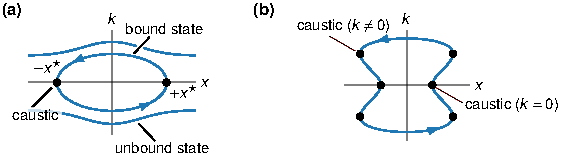
\includegraphics{localization/caustic.pdf}
  \end{center}
  \caption{%
    (a) In phase space, bound states are represented by rays in the form of closed orbits, which is analogous to that of a bound particle oscillating between two classical turning points ($\pm x^{\star}$ in the cartoon).
    Other trajectories represent unbound states.
    (b) A bound state represented by a ``peanut''-shaped orbit has six caustics.%
  }
  \label{fig:caustic}
\end{figure}
